\insertmeeting 
	{Formula 1 is Our Formula} 
	{10-6-22} 
	{Hagerty High School}
	{Anouska, Jensen, Jorge, Mohana, Nathan, Ritam, Robert, Tyler}
	{Images/RobotPics/robot.jpg}
	{2:30 - 8:30}
	
\hhscommittee{Hardware}
\noindent\hfil\rule{\textwidth}{.4pt}\hfil
\subsubsection*{Goals}
\begin{itemize}
    \item Address issue with steering linkage
    \item Understand mathematical principles behind Ackermann
    \item Create a new steering linkage that could balance simplicity and accuracy
    \item Add new steering linkage to drivetrain CAD

\end{itemize} 

\noindent\hfil\rule{\textwidth}{.4pt}\hfil

\subsubsection*{Accomplishments}
Unfortunately, before we could pursue our goals of finishing the back half of the drivetrain from the end of the last meeting, we encountered a fairly substantial issue that we had failed to consider before. In our Ackerman steering prototype, the two steering knuckles were connected together with a single tie bar which we thought would help the wheels turn in a perfect ackermann ratio, making each of them perfectly follow circles of different radii around the same center of rotation, resulting in a turn without any slippage. As it turns out, due to a missing constraint that was accidentally deleted from the Ackerman steering skeleton, the wheels do not follow a perfect ackermann ratio, instead driving on circular paths with different center points. Although the center points are consistently quite close together, some slipping may occur, making our autonomous inaccurate, unable to predictably go to the same location every time. Additionally, we noticed that the ackermann linkage used on the prototype, though it kept the wheels pointing in generally correct directions relative to each other, powering the linkage and making the robot steer from a servo would be very difficult due to the tie bar’s changing location and angle. All of these problems revealed an issue in how we had designed the prototype steering system. This issue was that we had only a surface-level understanding of ackermann and its applications, not truly knowing the math that causes ackermann steering linkages to work or comprehending the varieties of linkage setups which all have different purposed and priorities. 

Seeking to fix these issues, we started by looking into real world applications of Ackerman steering. Perhaps one of the reasons we hadn’t noticed the imperfection of our ackermann linkage was because most ackermann linkages aren’t perfect in the first place. For most applications, especially in the consumer automotive industry, a little bit of slippage when turning is hardly a problem. Any slipping that might occur is usually minimal and is easily corrected for by the driver without them even noticing. In several applications, perfect ackermann is even avoided. For example in Formula 1 race cars, a system called anti-ackermann is used, which makes the outer wheel turn more than the inner wheel (figure 1). This amount of error is created because of the high amount of downforce holding the cars to the race track, especially around corners where more force is put on the outer wheel. The greater turning angle caused by anti-ackermann allows the elite drivers of these race cars to get better rotation into a corner and better traction out of a corner. The reason that having as close to perfect ackermann as possible is so important for us when it isn’t important for consumer vehicles and F1 cars is because of our autonomous period. Because in real cars people are driving, any error from the Ackerman linkage can be corrected by the driver. On our robot during autonomous, the robot is being driven by a computer which has much more limited sensors than people have. Because of this, error caused by wheel slip can compound over the course of an autonomous period, making the robot go to a slightly different place every time. Although odometry could potentially be used to fix this, we want to minimize slippage as much as we can in hardware.
Another reason for our problems was our lack of understanding of the mathematics related to ackermann. To help fully understand how ackermann works and the relationship of the angle between the inner and outer wheel, we drew a diagram (figure 2) and used some trigonometry to describe the angle of each wheel as it relates to the turning radius (figure 3). Knowing these formulas allows us to verify and compare the perfect ackermann angle with the actual angle of our linkage.

To fix our problem, we started looking into variations of ackermann linkages that give perfect or almost perfect angles for both wheels. Finding several designs, we picked a few that we thought seemed promising and easy to reproduce at the small scale of our robot. Using these designs and a few of our own, we created about 15 sketches in onshape which allowed us to simulate the angle of the inner and outer wheels at different turning radii, which we then compared to the perfect angle of the inner and outer wheels given by the formula we derived earlier in the meeting some of the more notable designs we tested were bellcrank steering (figure 4) Davis steering (figure 5) and several unnamed variations from cars, go-carts, and RC cars (figures 6 and 7). After testing each design and weighing the simplicity of some designs and the ratio accuracy of others, we decided on a variation of the bell crank design, changing a few of the key measurements to maximize efficiency for our robot’s needs. This linkage was easy to implement with parts that aren’t too bulky or heavy, while still providing an ackermann ratio close enough to perfect to be negligible, if not fixable using a couple extra sensors. 

Unfortunately, before we could pursue our goals of finishing the back half of the drivetrain from the end of the last meeting, we encountered a fairly substantial issue that we had failed to consider before. In our Ackermann steering prototype, the two steering knuckles were connected together with a single tie bar which we thought would help the wheels turn in a perfect Ackermann ratio, making each of them perfectly follow circles of different radii around the same center of rotation, resulting in a turn without any slippage. As it turns out, due to a missing constraint that was accidentally deleted from the Ackermann steering skeleton, the wheels do not follow a perfect Ackermann ratio, instead driving on circular paths with different center points. Although the center points are consistently quite close together, some slipping may occur, making our autonomous inaccurate, unable to predictably go to the same location every time. Additionally, we noticed that the Ackermann linkage used on the prototype, though it kept the wheels pointing in generally correct directions relative to each other, powering the linkage and making the robot steer from a servo would be very difficult due to the tie bar’s changing location and angle. All of these problems revealed an issue in how we had designed the prototype steering system. This issue was that we had only a surface-level understanding of Ackermann and its applications, not truly knowing the math that causes Ackermann steering linkages to work or comprehending the varieties of linkage setups which all have different purposed and priorities. 
Seeking to fix these issues, we started by looking into real world applications of Ackermann steering. Perhaps one of the reasons we hadn’t noticed the imperfection of our Ackermann linkage was because most Ackermann linkages aren’t perfect in the first place. For most applications, especially in the consumer automotive industry, a little bit of slippage when turning is hardly a problem. Any slipping that might occur is usually minimal and is easily corrected for by the driver without them even noticing. In several applications, perfect Ackermann is even avoided. For example in Formula 1 race cars, a system called anti-Ackermann is used, which makes the outer wheel turn more than the inner wheel (figure 1). This amount of error is created because of the high amount of downforce holding the cars to the race track, especially around corners where more force is put on the outer wheel. The greater turning angle caused by anti-Ackermann allows the elite drivers of these race cars to get better rotation into a corner and better traction out of a corner. The reason that having as close to perfect Ackermann as possible is so important for us when it isn’t important for consumer vehicles and F1 cars is because of our autonomous period. Because in real cars people are driving, any error from the Ackermann linkage can be corrected by the driver. On our robot during autonomous, the robot is being driven by a computer which has much more limited sensors than people have. Because of this, error caused by wheel slip can compound over the course of an autonomous period, making the robot go to a slightly different place every time. Although odometry could potentially be used to fix this, we want to minimize slippage as much as we can in hardware.
Another reason for our problems was our lack of understanding of the mathematics related to Ackermann. To help fully understand how Ackermann works and the relationship of the angle between the inner and outer wheel, we drew a diagram (figure 2) and used some trigonometry to describe the angle of each wheel as it relates to the turning radius (figure 3). Knowing these formulas allows us to verify and compare the perfect Ackermann angle with the actual angle of our linkage.
To fix our problem, we started looking into variations of Ackermann linkages that give perfect or almost perfect angles for both wheels. Finding several designs, we picked a few that we thought seemed promising and easy to reproduce at the small scale of our robot. Using these designs and a few of our own, we created about 15 sketches in onshape which allowed us to simulate the angle of the inner and outer wheels at different turning radii, which we then compared to the perfect angle of the inner and outer wheels given by the formula we derived earlier in the meeting some of the more notable designs we tested were bellcrank steering (figure 4) Davis steering (figure 5) and several unnamed variations from cars, go-carts, and RC cars (figures 6 and 7). After testing each design and weighing the simplicity of some designs and the ratio accuracy of others, we decided on a variation of the bell crank design, changing a few of the key measurements to maximize efficiency for our robot’s needs. This linkage was easy to implement with parts that aren’t too bulky or heavy, while still providing an Ackermann ratio close enough to perfect to be negligible, if not fixable using a couple extra sensors. 

We used ball joint linkages, a part common on rc cars, to connect the steering knuckles to a servo. We added all of this into CAD, including a laser cut platform that would allow us to easily change the size or location of the servo if we needed to in the future without requiring us to reprint the entire drivetrain. We then made an assembly including all of the linkage parts (figure 8), ensuring that the wheels could turn to the correct angles according to the equations we derived. 


\begin{figure}[ht]
\centering
\begin{minipage}[b]{.48\textwidth}
  \centering
  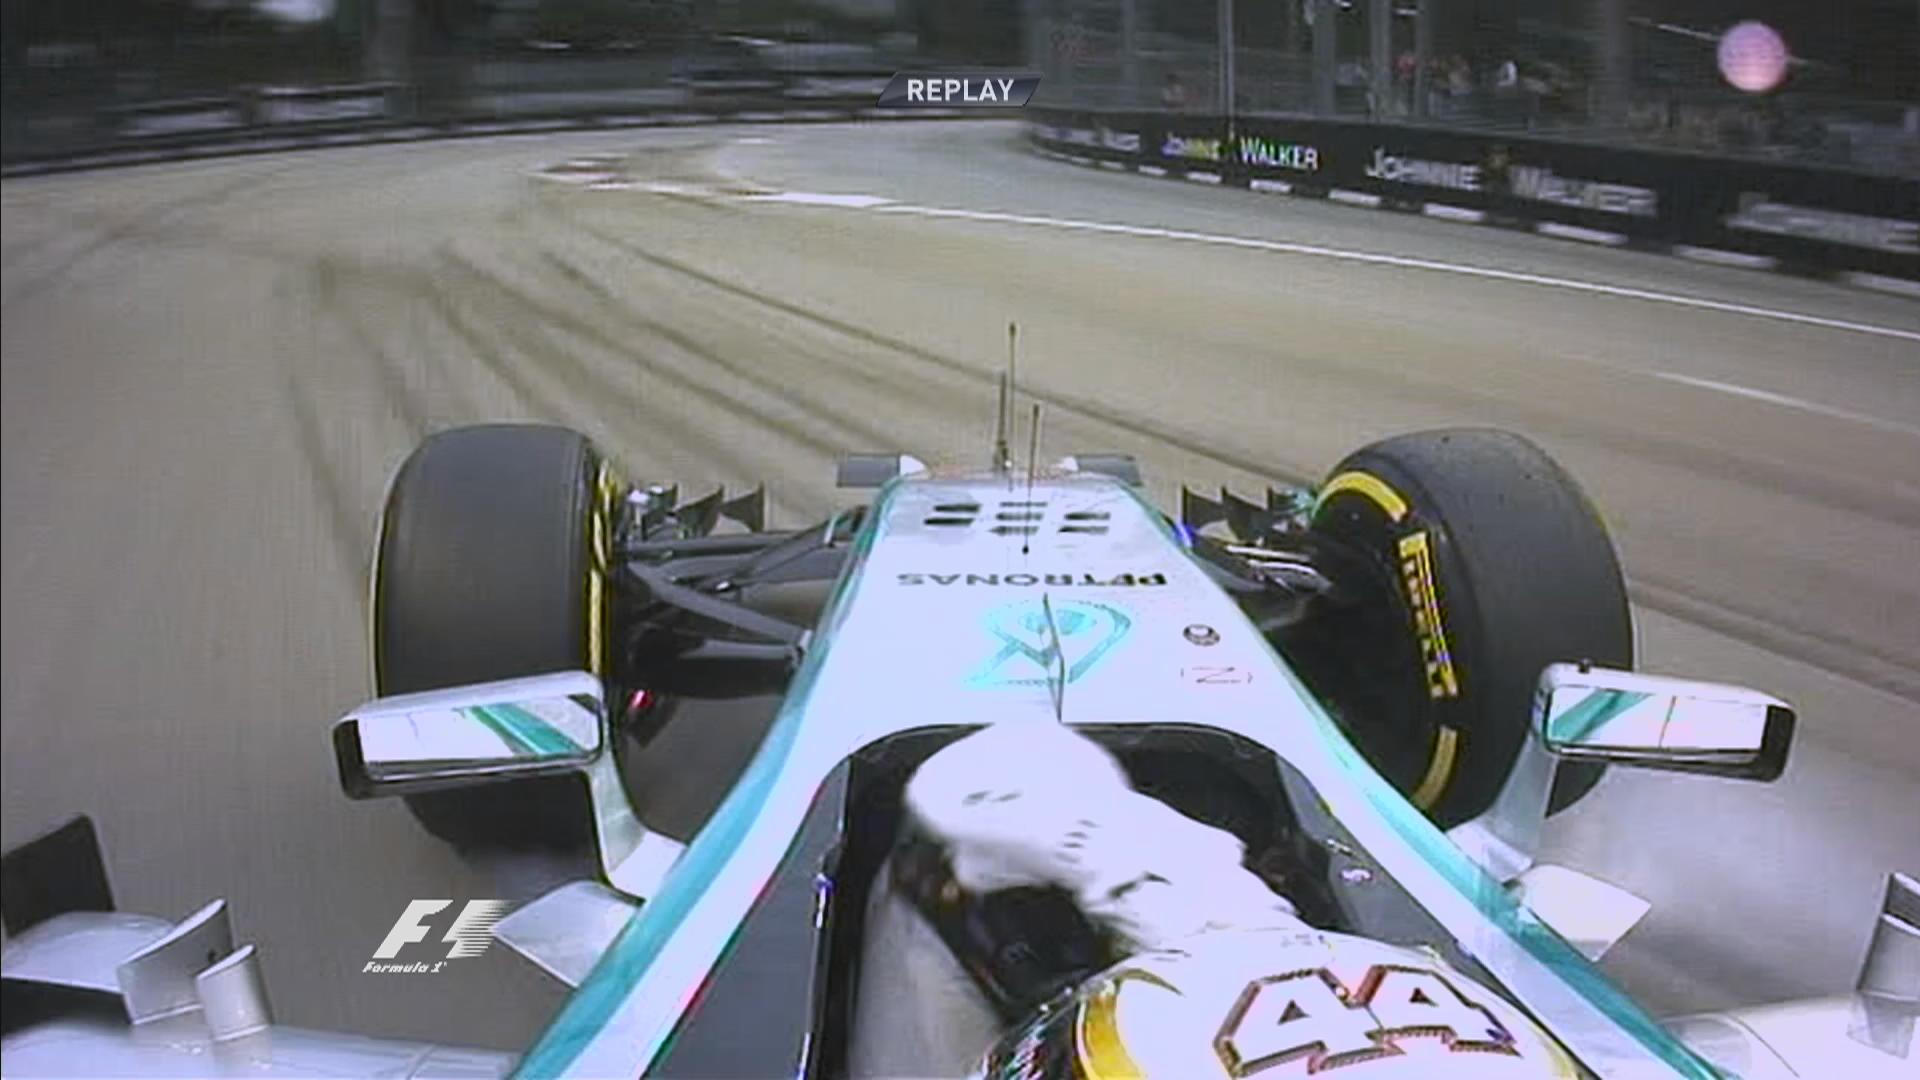
\includegraphics[width=0.95\textwidth]{Meetings/October/10-06-22/10-6-22_CAD_Figure1.jpg}
  \caption{Real example of how Ackermann steering is usedin cars}
  \label{fig:pic1}
\end{minipage}%
\hfill%
\begin{minipage}[b]{.48\textwidth}
  \centering
  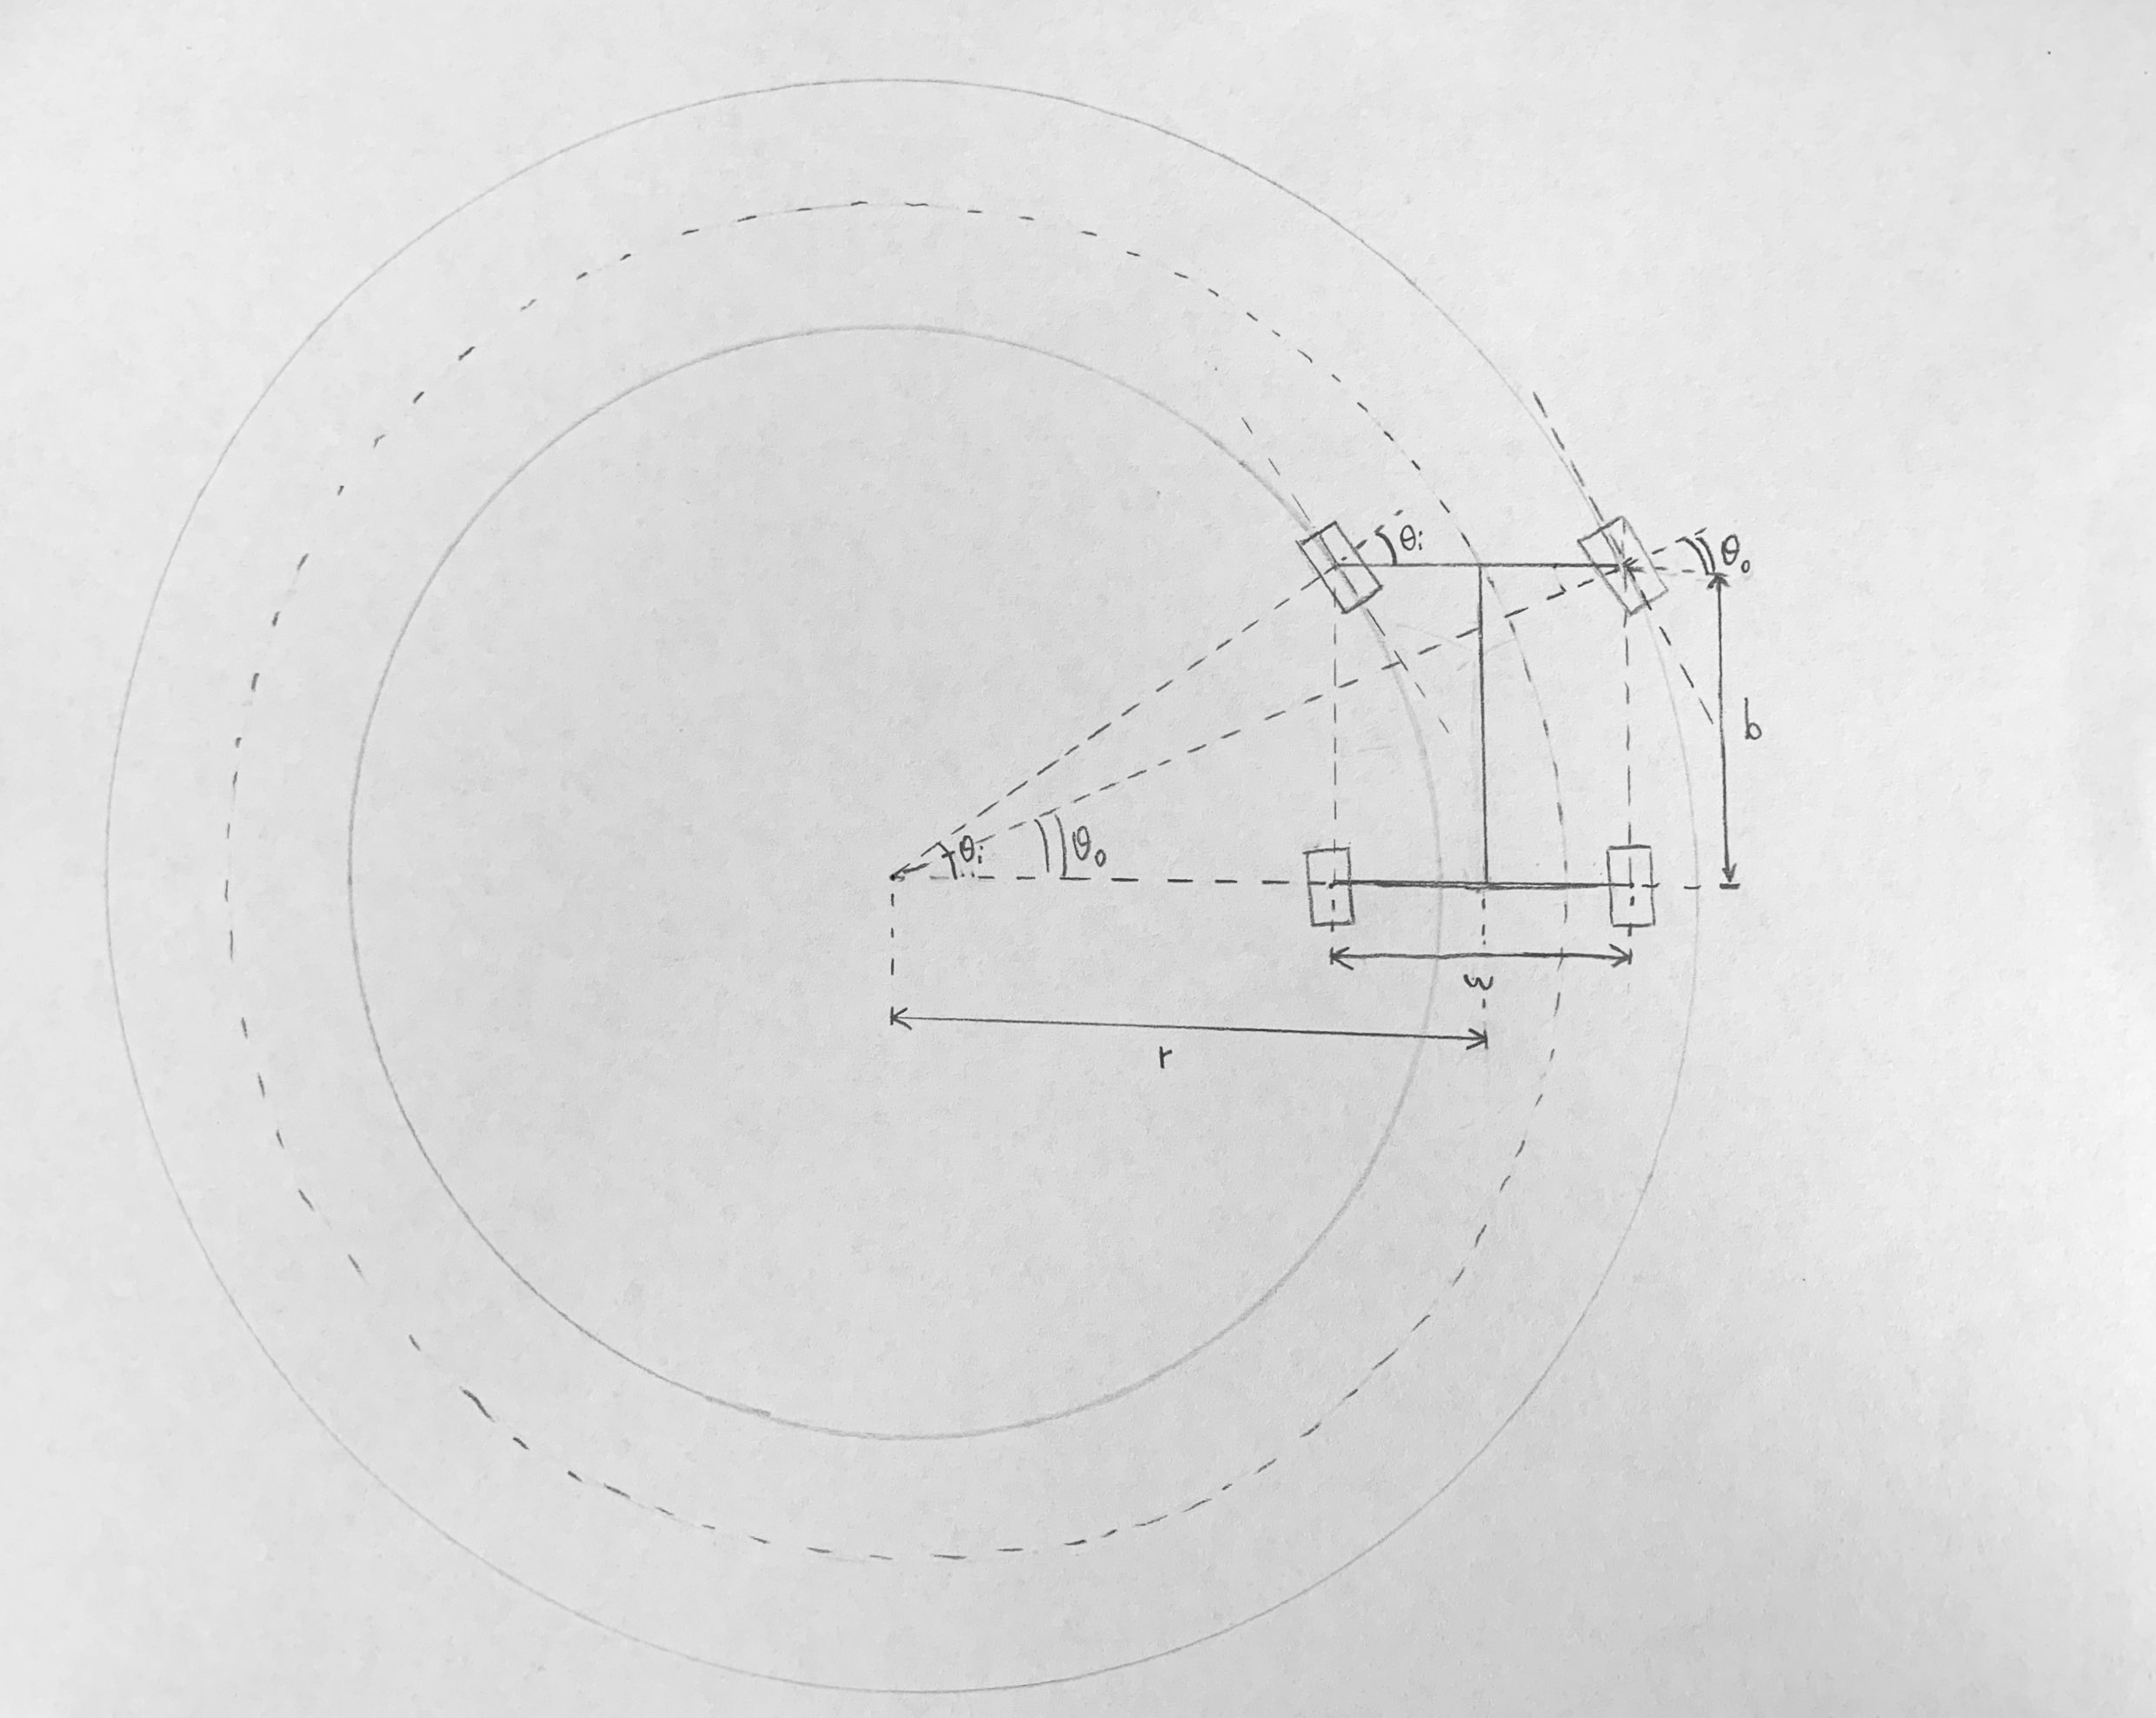
\includegraphics[width=0.95\textwidth]{Meetings/October/10-06-22/10-6-22_CAD_Figure3.png}
  \caption{4717 robot from 2021-2022 season}
  \label{fig:pic2}
\end{minipage}
\end{figure}

\begin{figure}[ht]
\centering
\begin{minipage}[b]{.48\textwidth}
  \centering
  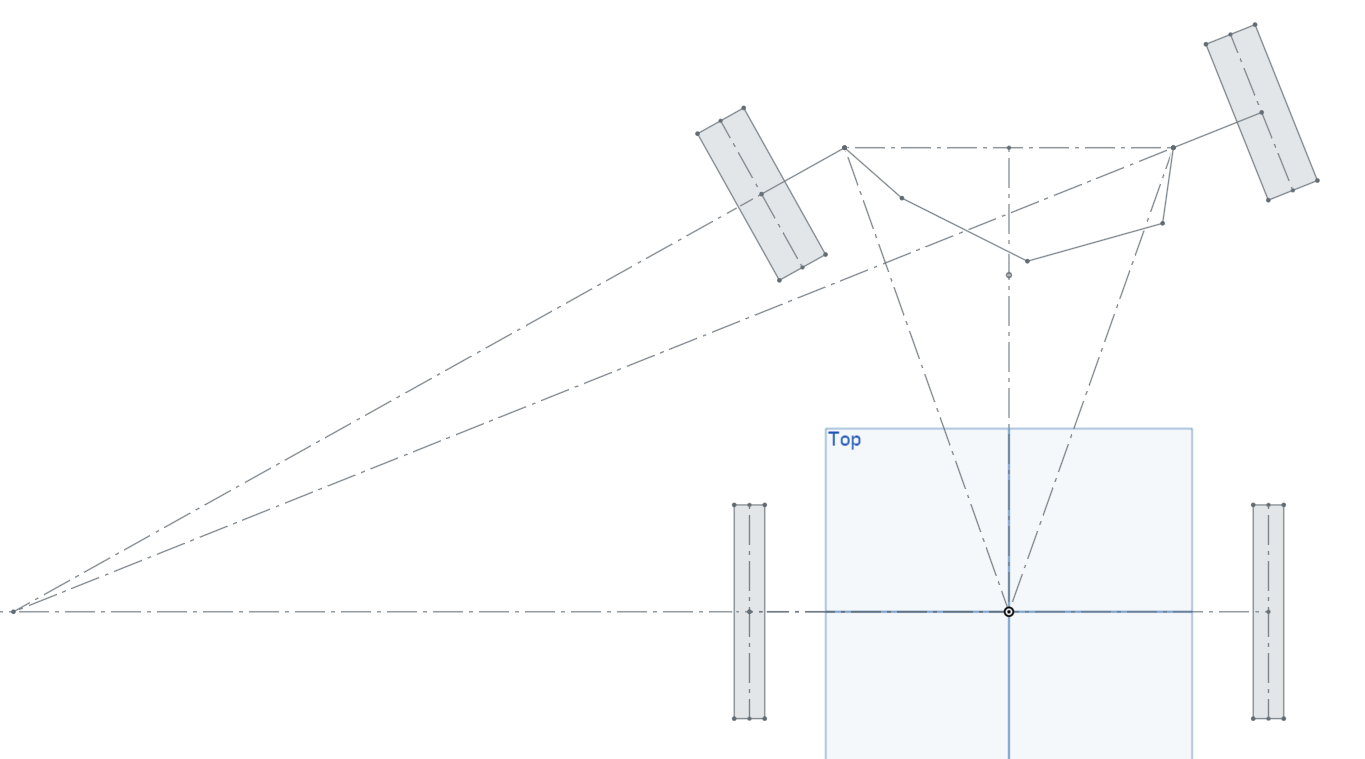
\includegraphics[width=0.95\textwidth]{Meetings/October/10-06-22/10-6-22_CAD_Figure4.PNG}
  \caption{4227 robot from 2021-2022 season}
  \label{fig:pic1}
\end{minipage}%
\hfill%
\begin{minipage}[b]{.48\textwidth}
  \centering
  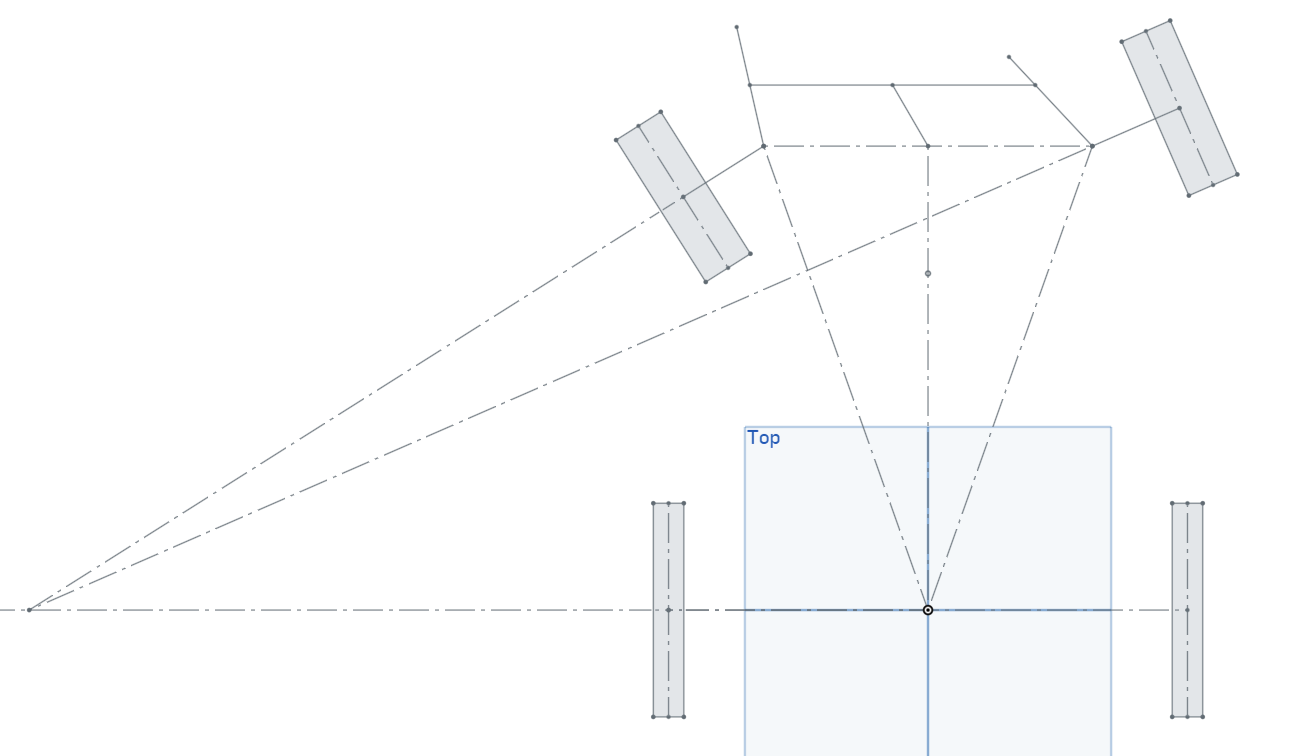
\includegraphics[width=0.95\textwidth]{Meetings/October/10-06-22/10-6-22_CAD_Figure5.PNG}
  \caption{4717 robot from 2021-2022 season}
  \label{fig:pic2}
\end{minipage}
\end{figure}



\whatsnext{
\begin{itemize}
    \item Complete back half of drivetrain
    \item Print drivetrain
    \item Start on intake mechanism
    
\end{itemize} 
}
